\begin{flushleft}

\chapter{Working on Avrdude (Linux Platform)}



\medskip
Hello world ! This is a quick tutorial for working on Avrdude on the linux platform. This chapter covers the installation of Avrdude and other necessary software followed by compiling a program, generating a .hex file and loading the .hex file to the Atmega2560 controller using stk500v2 programmer. Refer to \cite{installation}\cite{loading}\cite{binutils}\cite{avr-libc}\cite{avrdude}



\section{\textbf{Installation Procedure}}

\subsection{Unix setup paths}
\textbf{Step 1 : }
\medskip

Open a new terminal and type - 


\medskip

\framebox{\parbox{\dimexpr\linewidth-2\fboxsep-2\fboxrule}{echo \$SHELL}}
\medskip

Press return.
\medskip

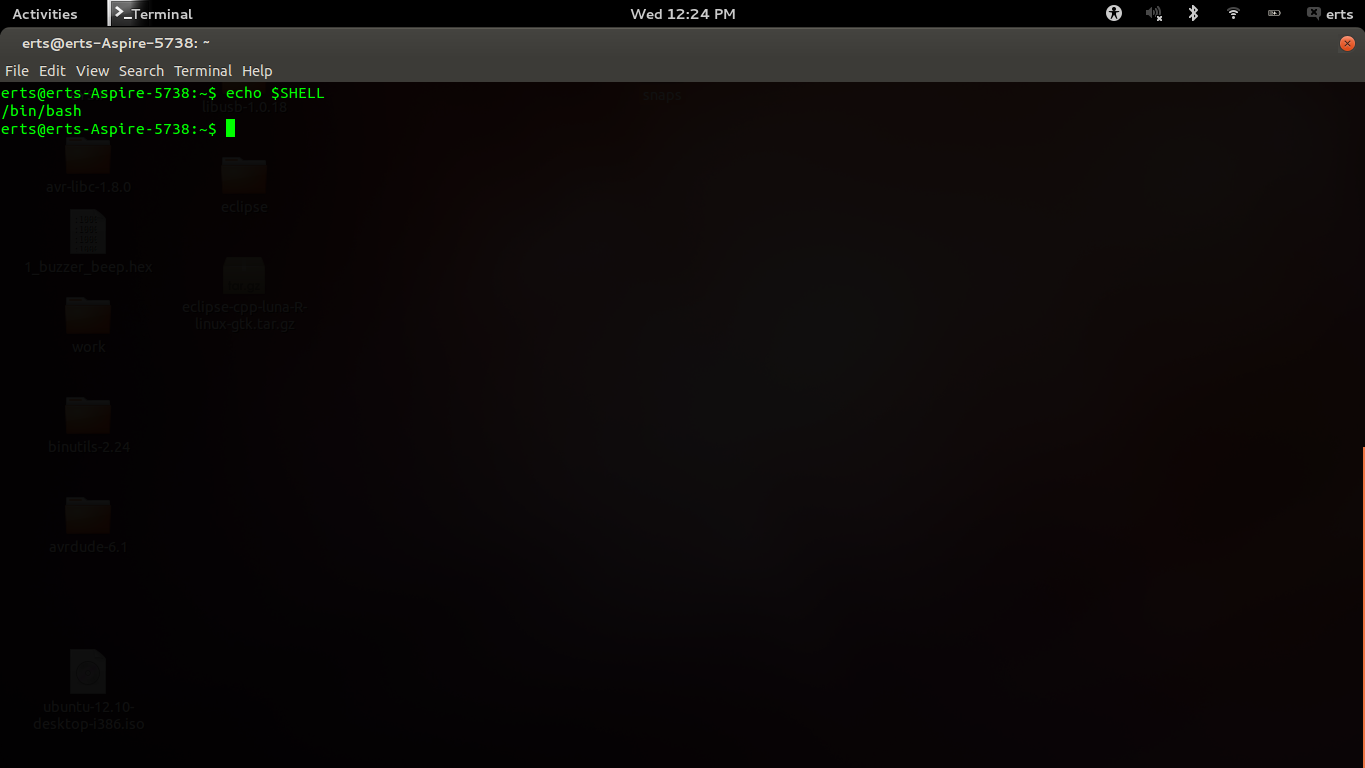
\includegraphics[scale=0.3]{f1}

\medskip

\textbf{Step 2 :}

\medskip

If the output is \textbf{/bin/bash} then type the following command:
\medskip

\framebox{\parbox{\dimexpr\linewidth-2\fboxsep-2\fboxrule}{echo 'PATH=\$PATH:/usr/local/bin' $>$$>$ \textasciitilde/.bash\_profile}}
\medskip

Press return.

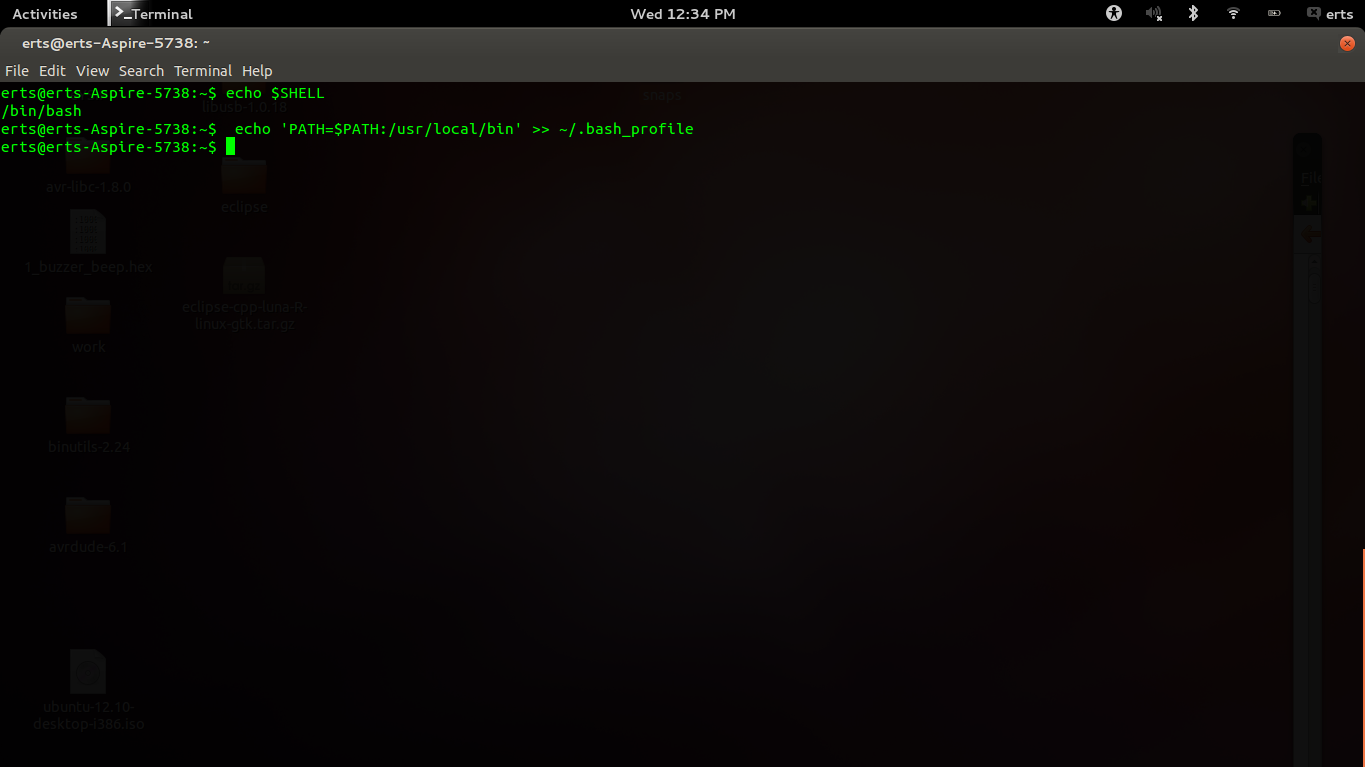
\includegraphics[scale=0.3]{f2}

\medskip

If the output is \textbf{/bin/csh} or \textbf{/bin/tcsh} then type the following command:

\medskip

\framebox{\parbox{\dimexpr\linewidth-2\fboxsep-2\fboxrule}{echo 'set path = (\$path /usr/local/bin)' $>$$>$ \textasciitilde/.cshrc}}
\medskip

Press return. 


\medskip

\textbf{Step 3 :}

\medskip

Close any open terminals and open a new one.

Now type :

\medskip

\framebox{\parbox{\dimexpr\linewidth-2\fboxsep-2\fboxrule}{echo \$PATH}}

\medskip

You should get an output similar to the one shown :
\medskip

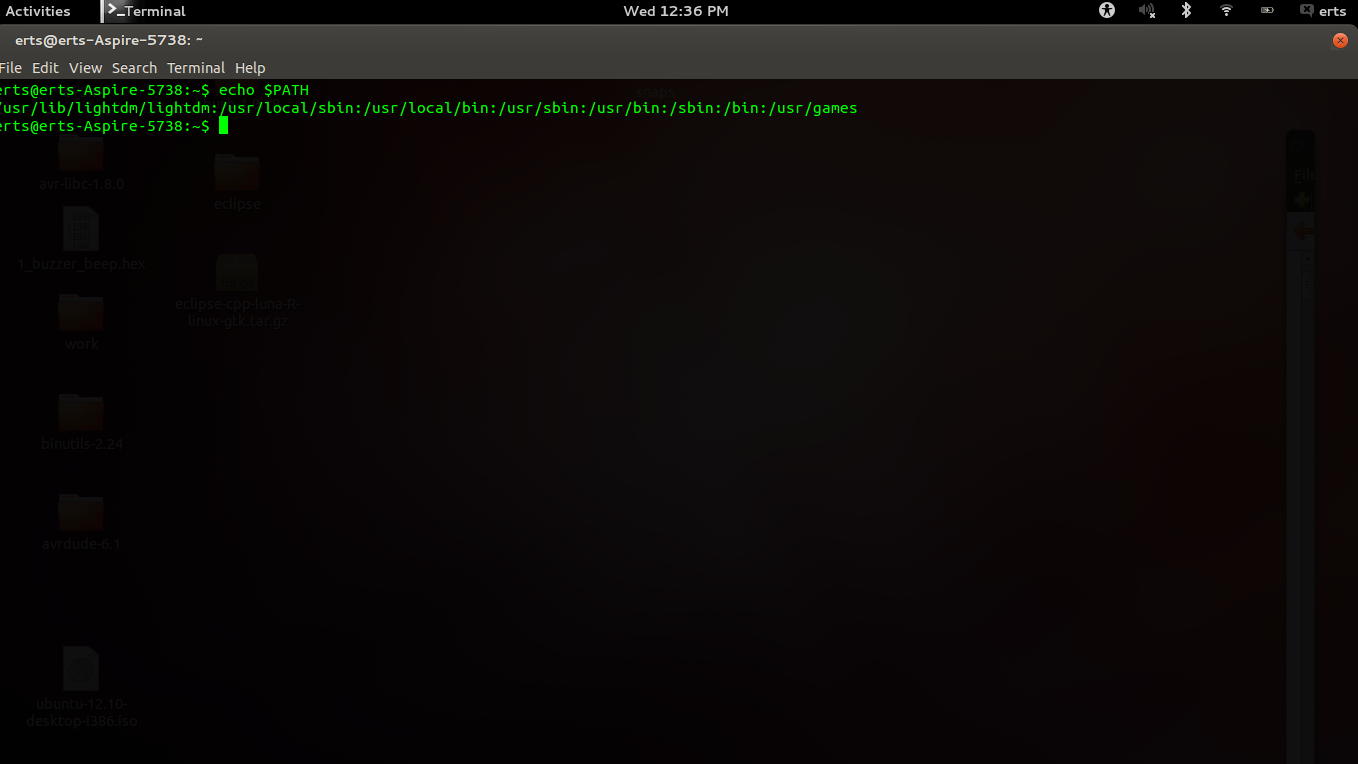
\includegraphics[scale=0.3]{f3}

\medskip

The important thing is that somewhere in the line of text you see \textbf{/usr/local/bin}.
\medskip



\subsection{Download and install the developer tools }

\textbf{Step 1 : }

You'll need the following packages: flex, byacc, bison, gcc, libusb and libusb-dev (for USB avr programmers) 
So type - 

\medskip

\framebox{\parbox{\dimexpr\linewidth-2\fboxsep-2\fboxrule}{sudo apt-get install flex byacc bison gcc libusb-dev }}

\medskip

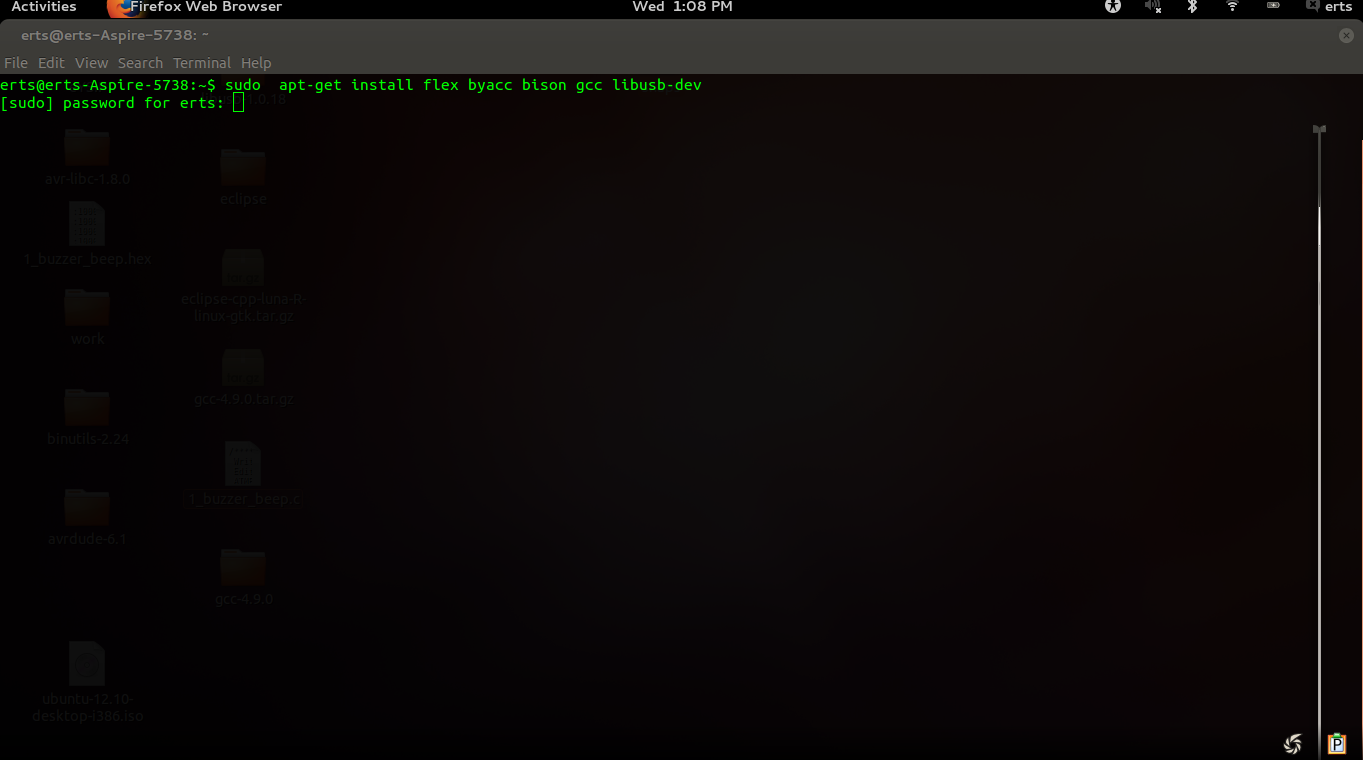
\includegraphics[scale=0.3]{f4}

\medskip

\subsection{Download \& install binutils}
\textbf{Step 1 : }
\medskip

Download the latest release of binutils from - 

\url{http://ftp.gnu.org/gnu/binutils/}

\medskip

Navigate to the binutils directory by typing - 

\medskip

\framebox{\parbox{\dimexpr\linewidth-2\fboxsep-2\fboxrule}{cd binutils-x.yz}}

\medskip

Configure binutils for AVR. by typing - 
\medskip

\framebox{\parbox{\dimexpr\linewidth-2\fboxsep-2\fboxrule}{./configure --target=avr --program-prefix="avr-"}}

\medskip

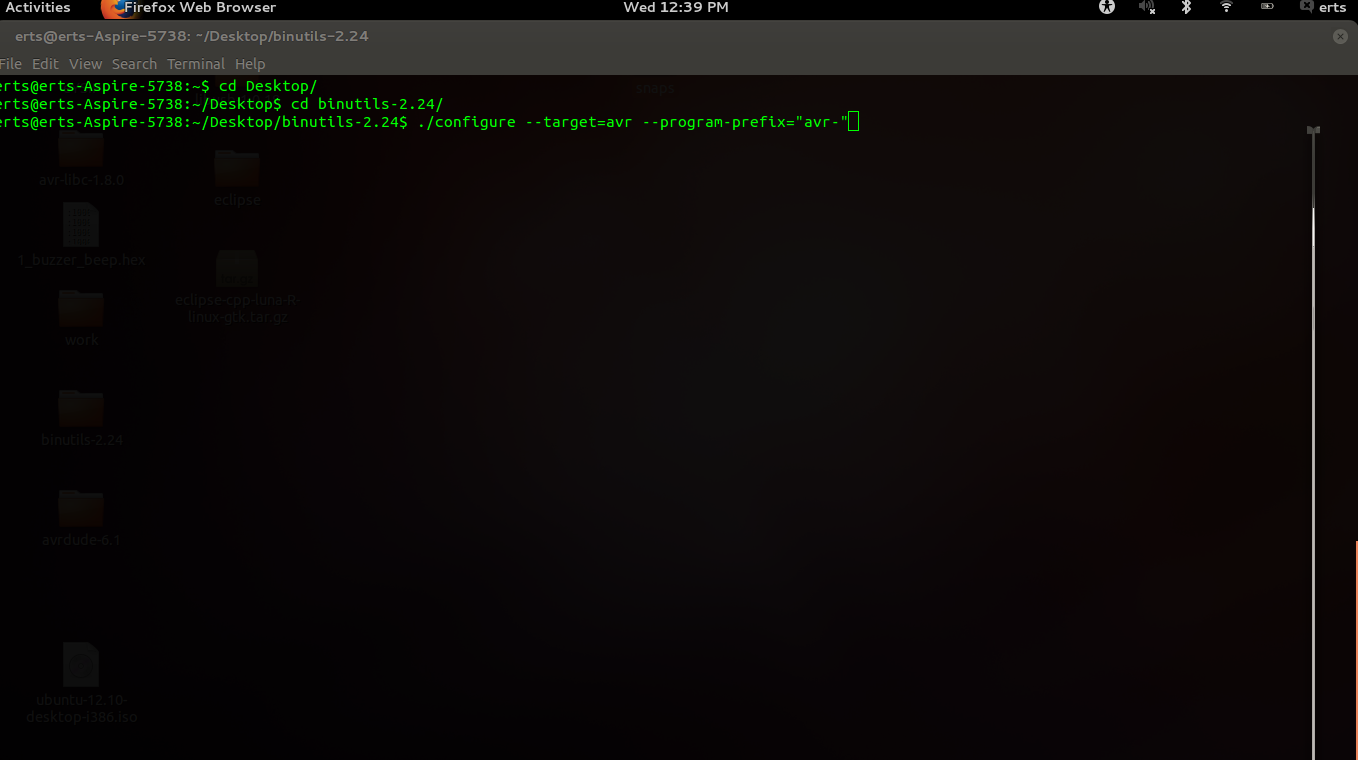
\includegraphics[scale=0.3]{f5}

\medskip

After completion you will see the following text - 

\medskip

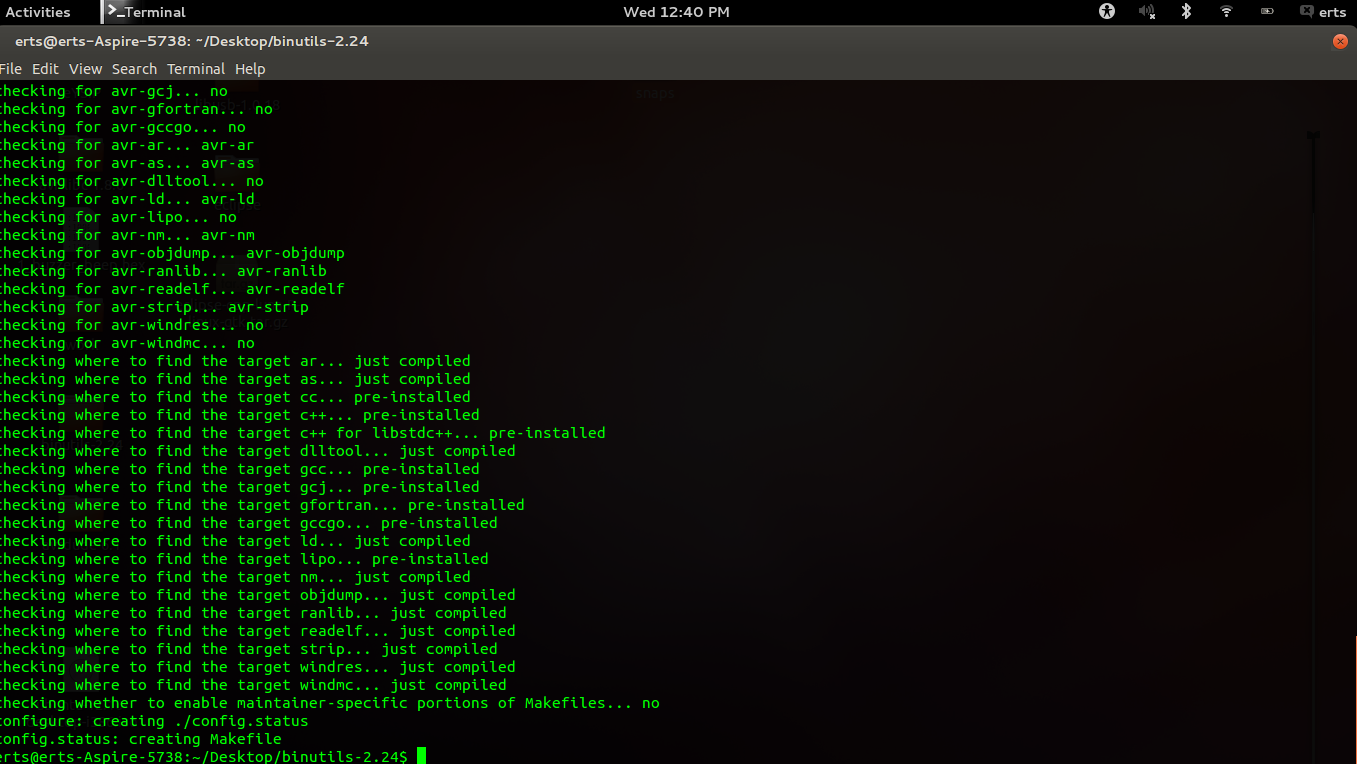
\includegraphics[scale=0.3]{f6}

\medskip

\textbf{Step 2 :}

\medskip

Compile binutils by typing - 
\medskip

\framebox{\parbox{\dimexpr\linewidth-2\fboxsep-2\fboxrule}{make}}
\medskip

Press return.

\medskip

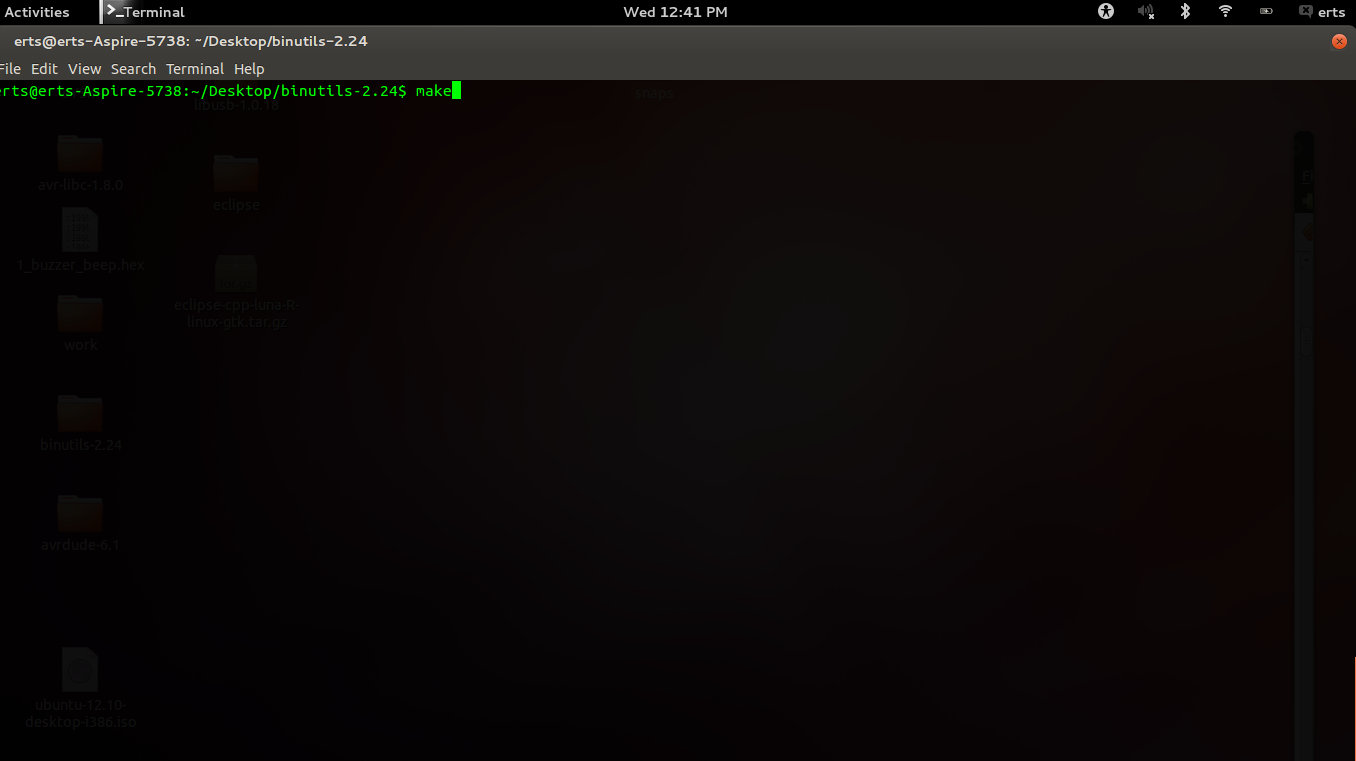
\includegraphics[scale=0.3]{f7}


\medskip

\textbf{Step 3 :}
 
Now install binutils by typing - 

\medskip

\framebox{\parbox{\dimexpr\linewidth-2\fboxsep-2\fboxrule}{sudo make install}}

\medskip

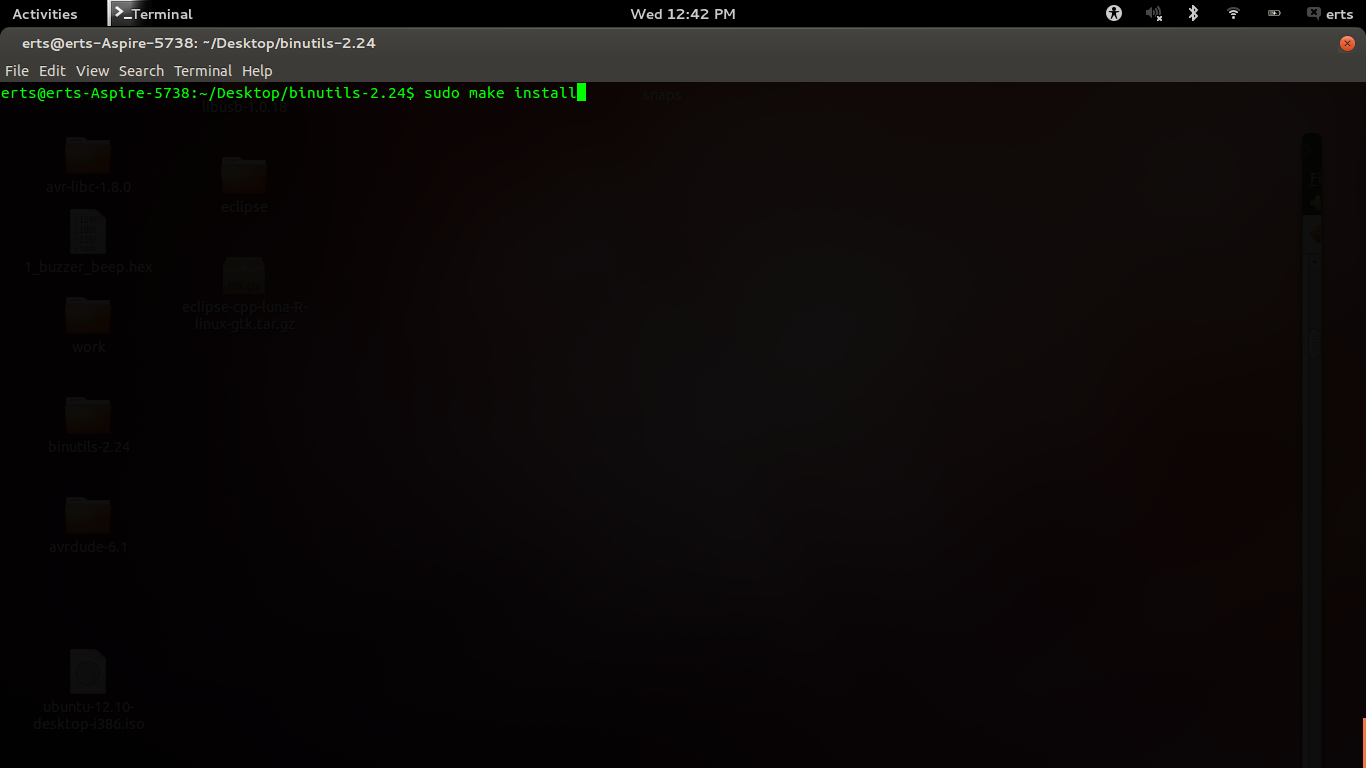
\includegraphics[scale=0.3]{f8}

\medskip

\subsection{Download and install avr-libc}

\textbf{Step 1 : }

\medskip

Download the current release of avr-libc from -

\url{http://savannah.nongnu.org/projects/avr-libc/}

\medskip

Navigate to the avr-libc directory by typing - 

\medskip

\framebox{\parbox{\dimexpr\linewidth-2\fboxsep-2\fboxrule}{cd avr-libc-x.y.z}}

\medskip

Configure avr-libc for AVR. by typing - 
\medskip

\framebox{\parbox{\dimexpr\linewidth-2\fboxsep-2\fboxrule}{./configure --host=avr}}

\medskip

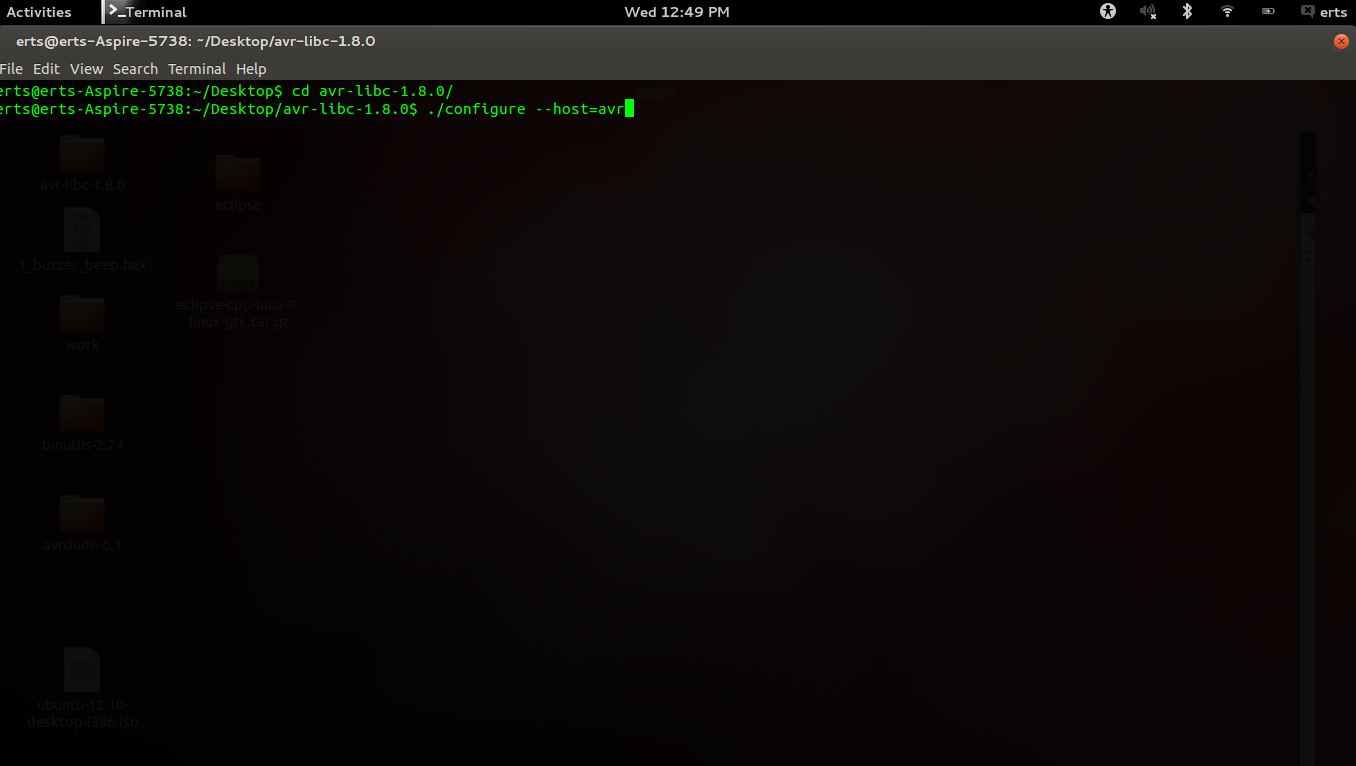
\includegraphics[scale=0.3]{f12}

\medskip

After completion you will see the following text - 

\medskip

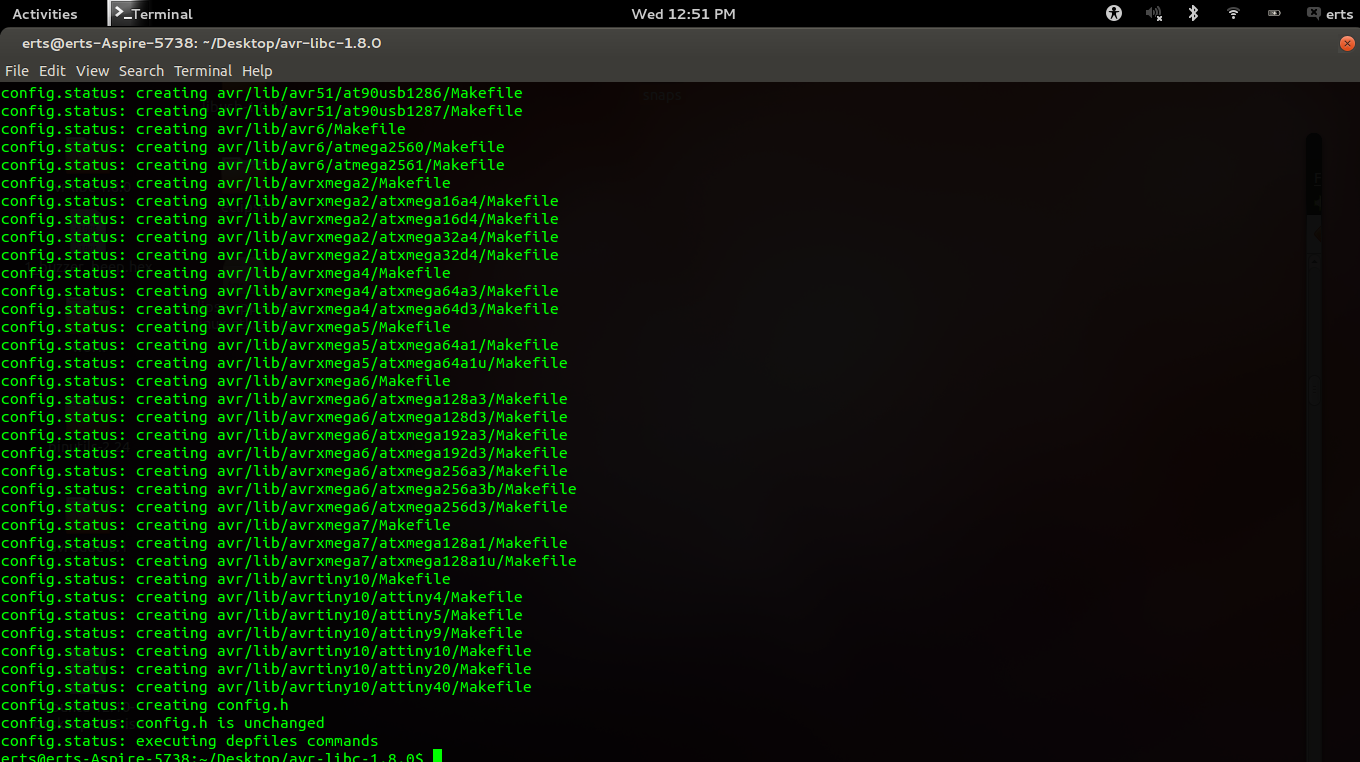
\includegraphics[scale=0.3]{f13}

\medskip

\textbf{Step 2 :}

\medskip

Compile binutils by typing - 
\medskip

\framebox{\parbox{\dimexpr\linewidth-2\fboxsep-2\fboxrule}{make}}
\medskip

Press return.

\medskip

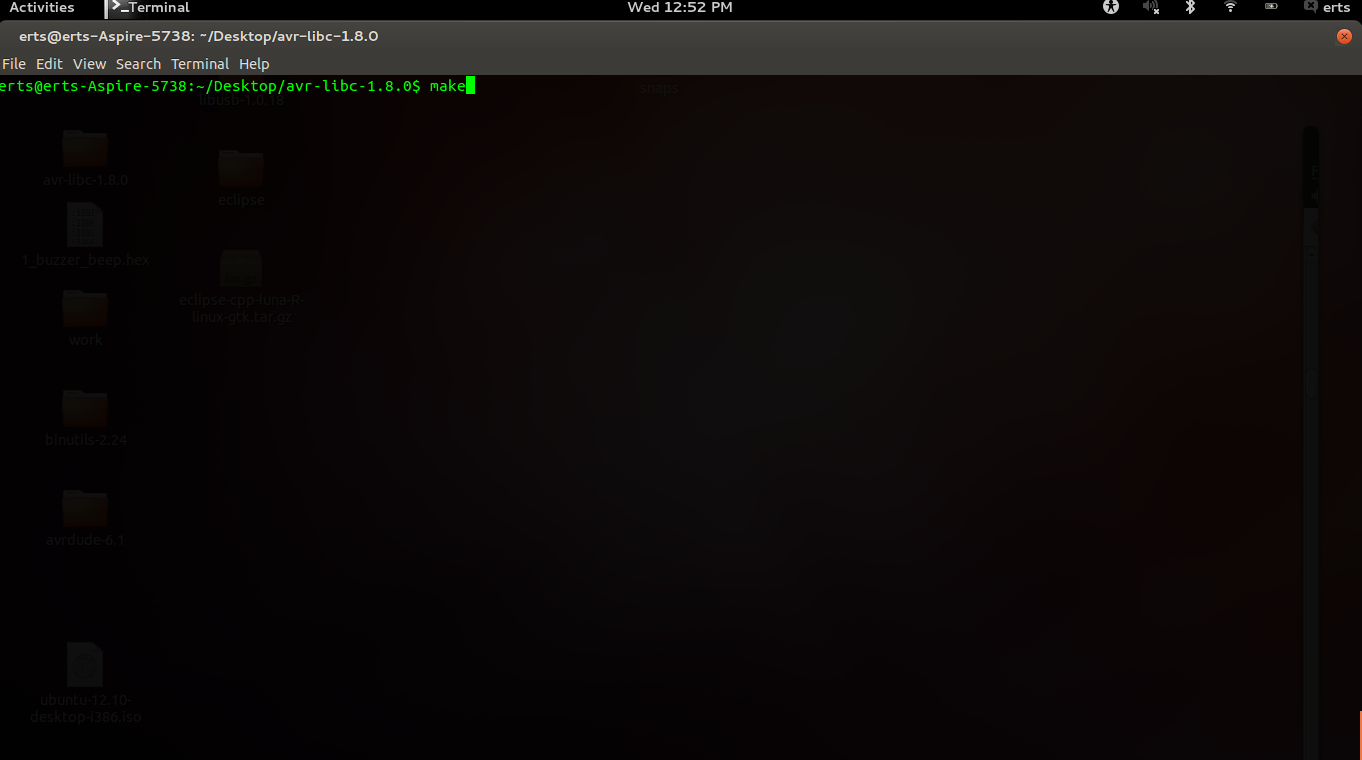
\includegraphics[scale=0.3]{f14}


\medskip

After completion you will see the following text - 

\medskip

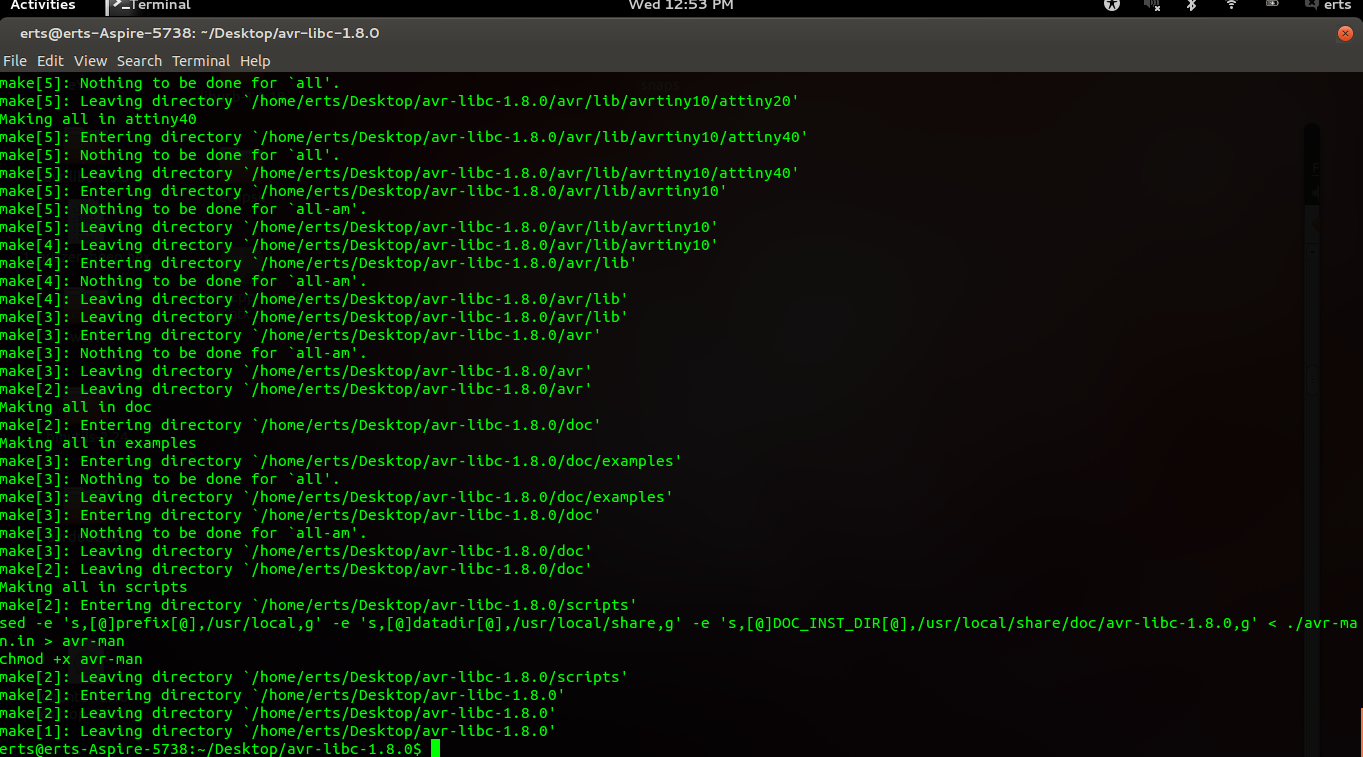
\includegraphics[scale=0.3]{f15}

\medskip

\textbf{Step 3 :}
 
Now install avr-libc by typing - 

\medskip

\framebox{\parbox{\dimexpr\linewidth-2\fboxsep-2\fboxrule}{sudo make install}}

\medskip

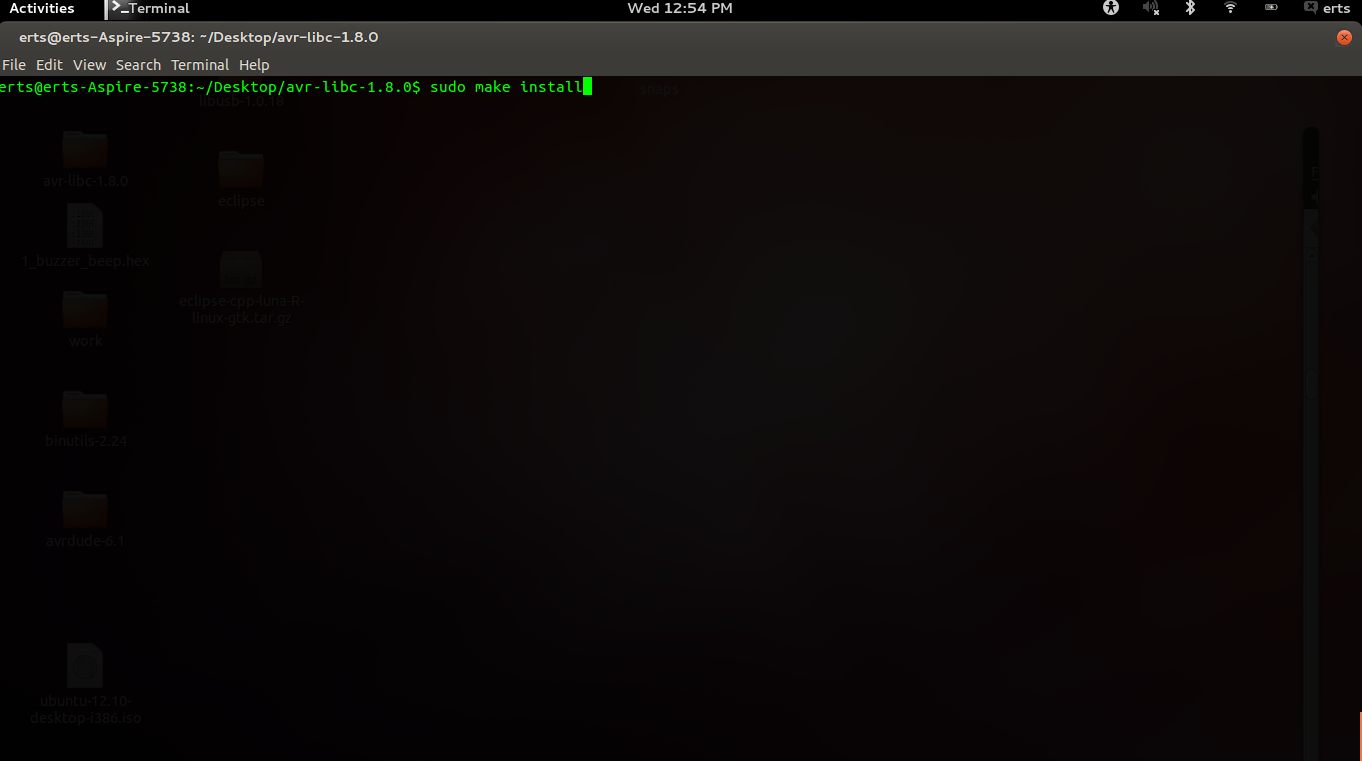
\includegraphics[scale=0.3]{f16}

\medskip

After completion you will see the following text - 

\medskip

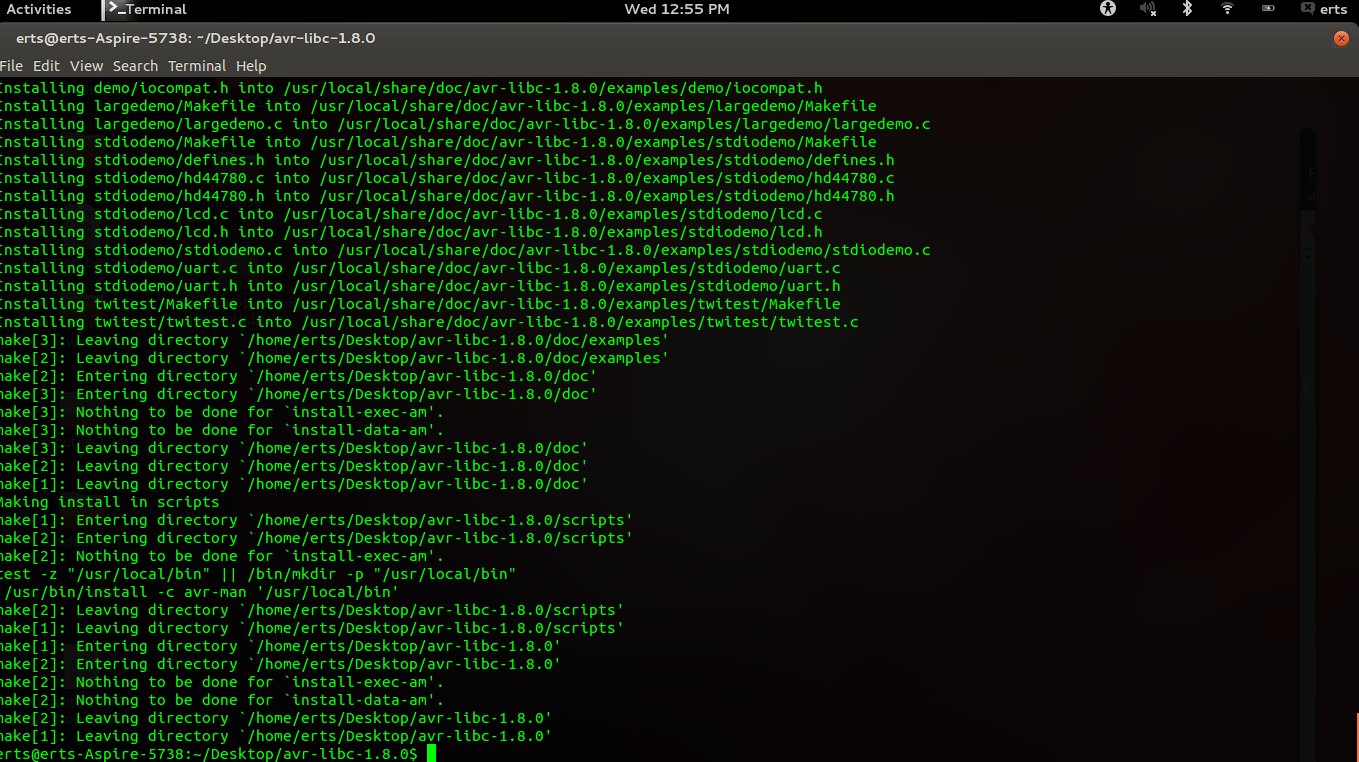
\includegraphics[scale=0.3]{f17}

\medskip

\subsection{Download and install avrdude}

\textbf{Step 1 : }

\medskip

Download the current release of avrdude from -

\url{http://download.savannah.gnu.org/releases/avrdude/}

\medskip

Navigate to the avrdude directory by typing - 

\medskip

\framebox{\parbox{\dimexpr\linewidth-2\fboxsep-2\fboxrule}{cd avrdude-x.yz}}

\medskip

Configure avrdude by typing - 
\medskip

\framebox{\parbox{\dimexpr\linewidth-2\fboxsep-2\fboxrule}{./configure}}

\medskip

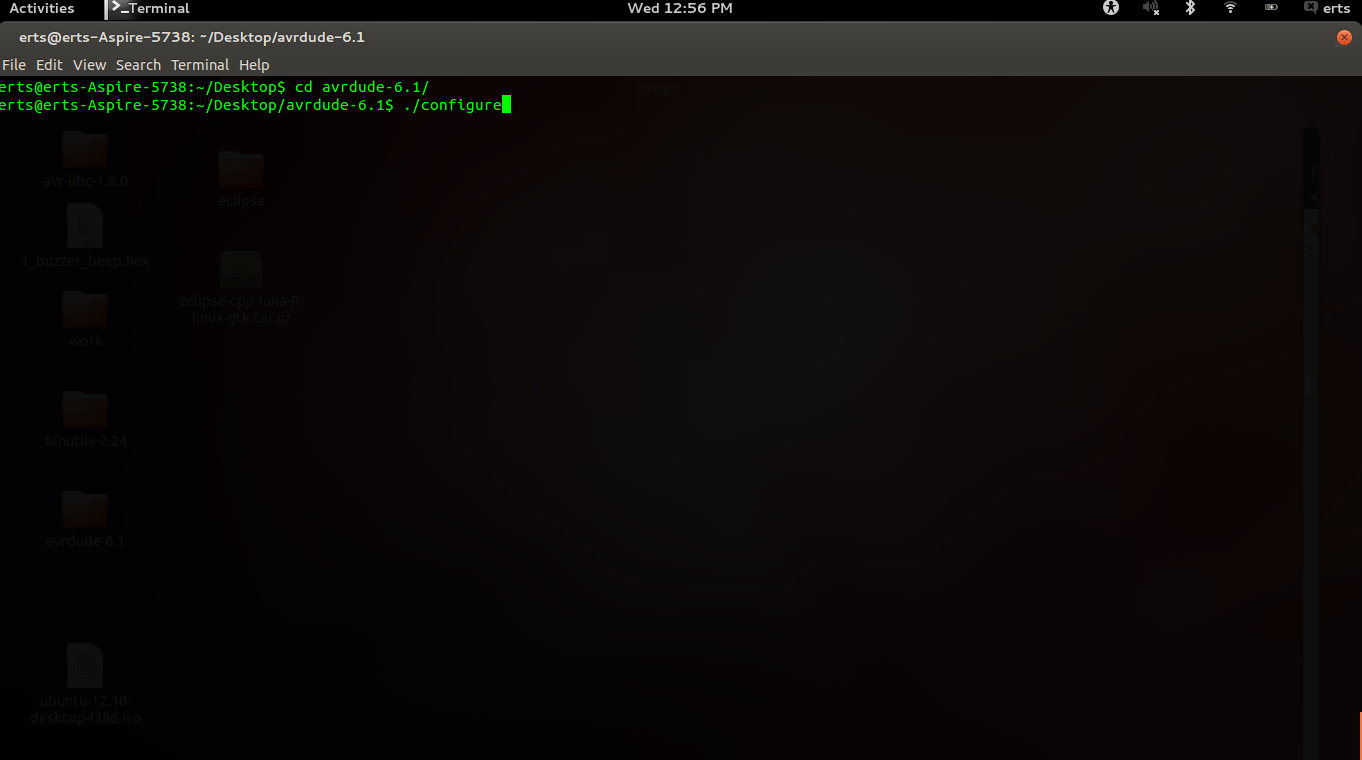
\includegraphics[scale=0.3]{f18}

\medskip

After completion you will see the following text - 

\medskip

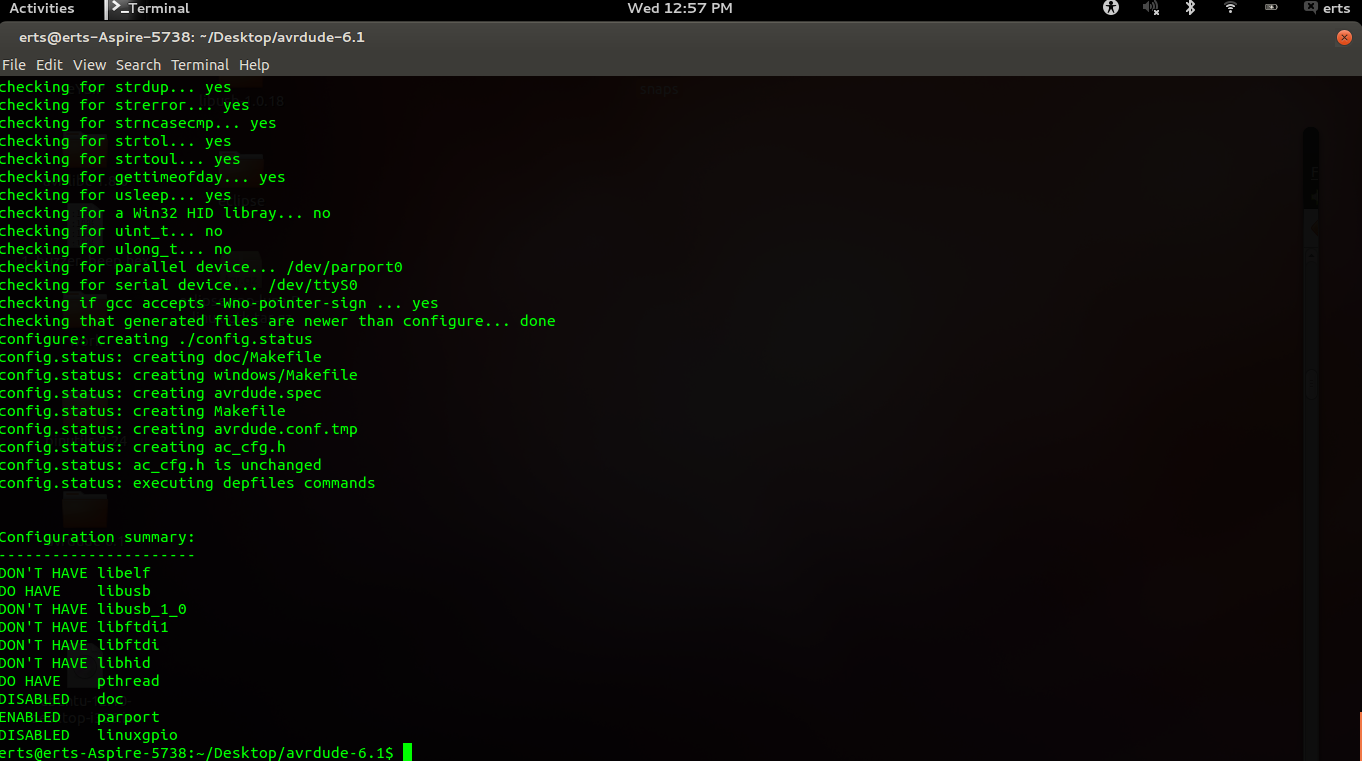
\includegraphics[scale=0.3]{f19}

\medskip

\textbf{Step 2 :}

\medskip

Compile avrdude by typing - 
\medskip

\framebox{\parbox{\dimexpr\linewidth-2\fboxsep-2\fboxrule}{make}}
\medskip

Press return.

\medskip

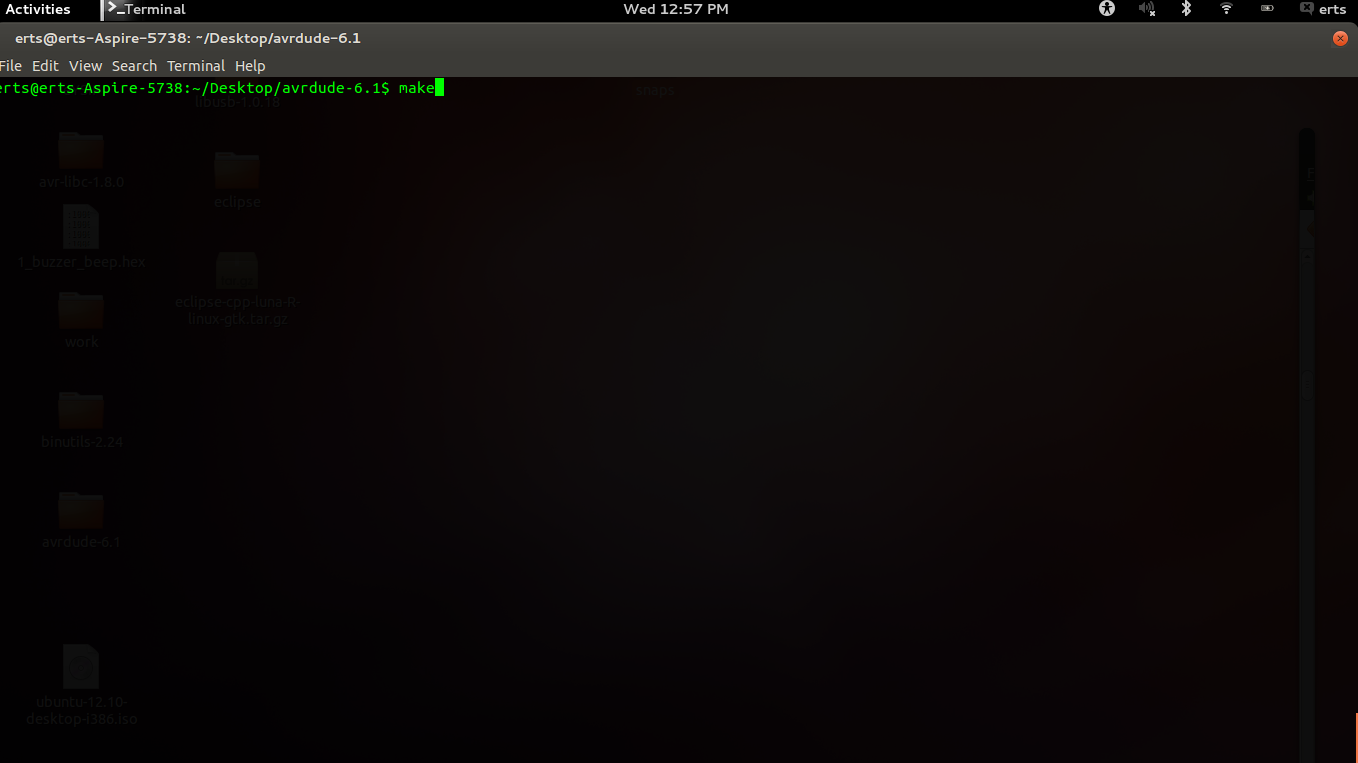
\includegraphics[scale=0.3]{f20}


\medskip

\textbf{Step 3 :}
 
Now install avrdude by typing - 

\medskip

\framebox{\parbox{\dimexpr\linewidth-2\fboxsep-2\fboxrule}{sudo make install}}

\medskip

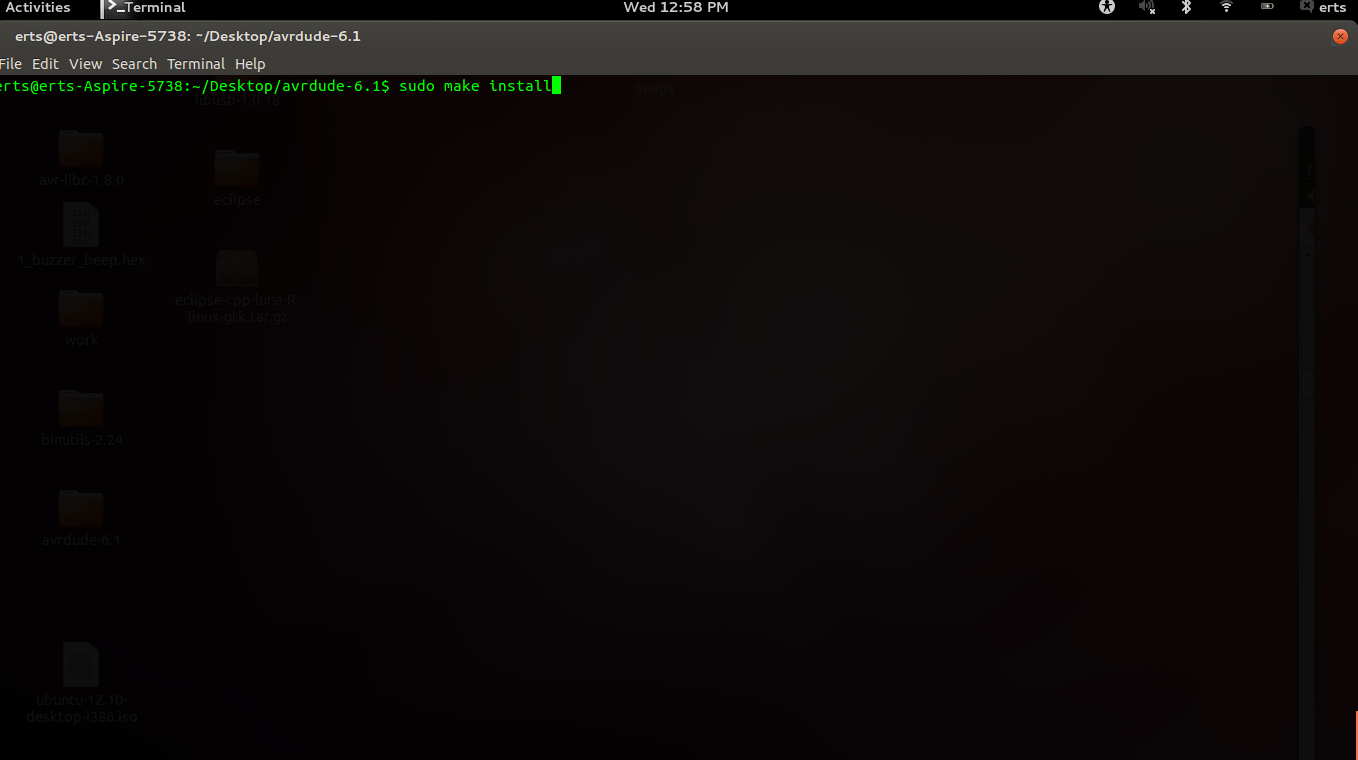
\includegraphics[scale=0.3]{f21}

\medskip

After completion you will see the following text - 

\medskip

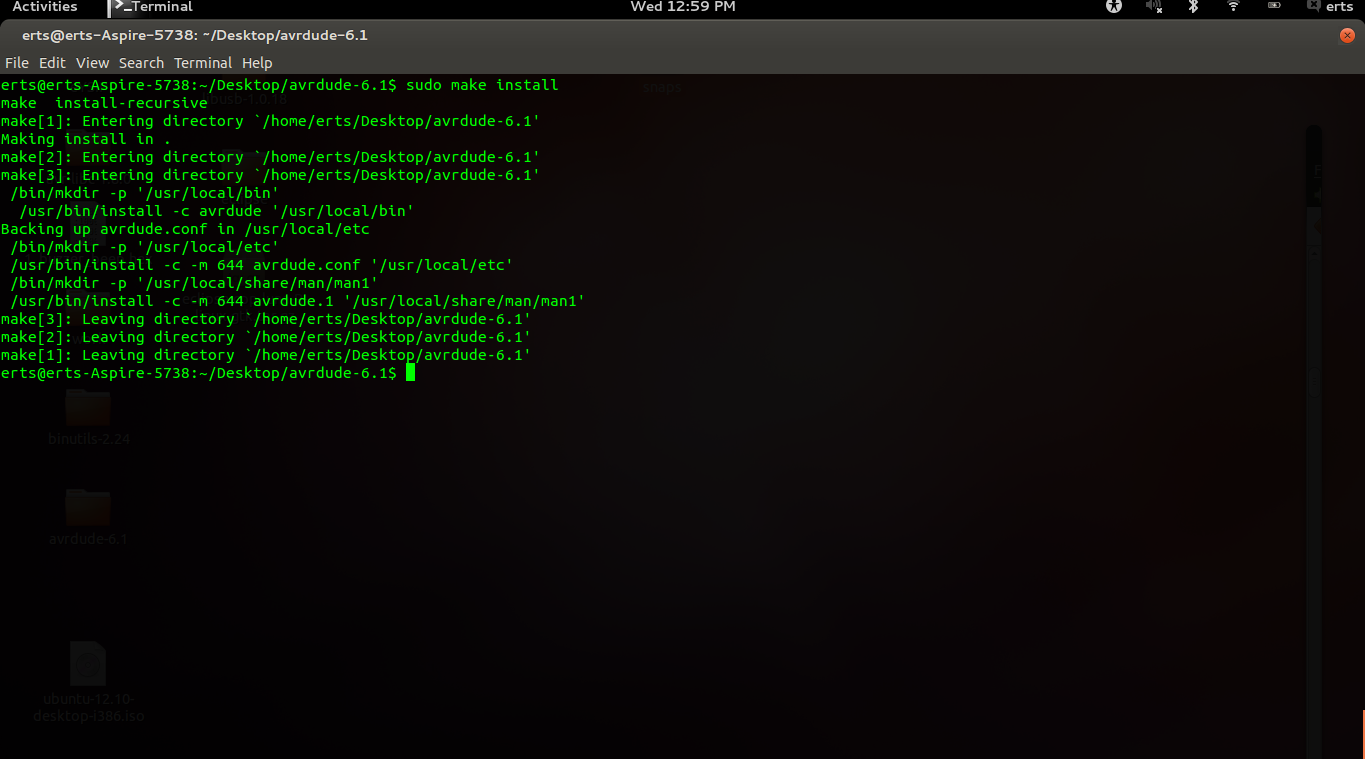
\includegraphics[scale=0.3]{f22}

\medskip

\section{\textbf{Compilation, Generation and loading of .hex file}}

Type a program for the AVR platform on gedit text editor and save the file with \textbf{.c} extension.

\subsection{Compilation}

\medskip

To compile the program type - 

\medskip

\framebox{\parbox{\dimexpr\linewidth-2\fboxsep-2\fboxrule}{avr-gcc -mmcu=atmega2560 filename.c -o some\_name}}

\medskip

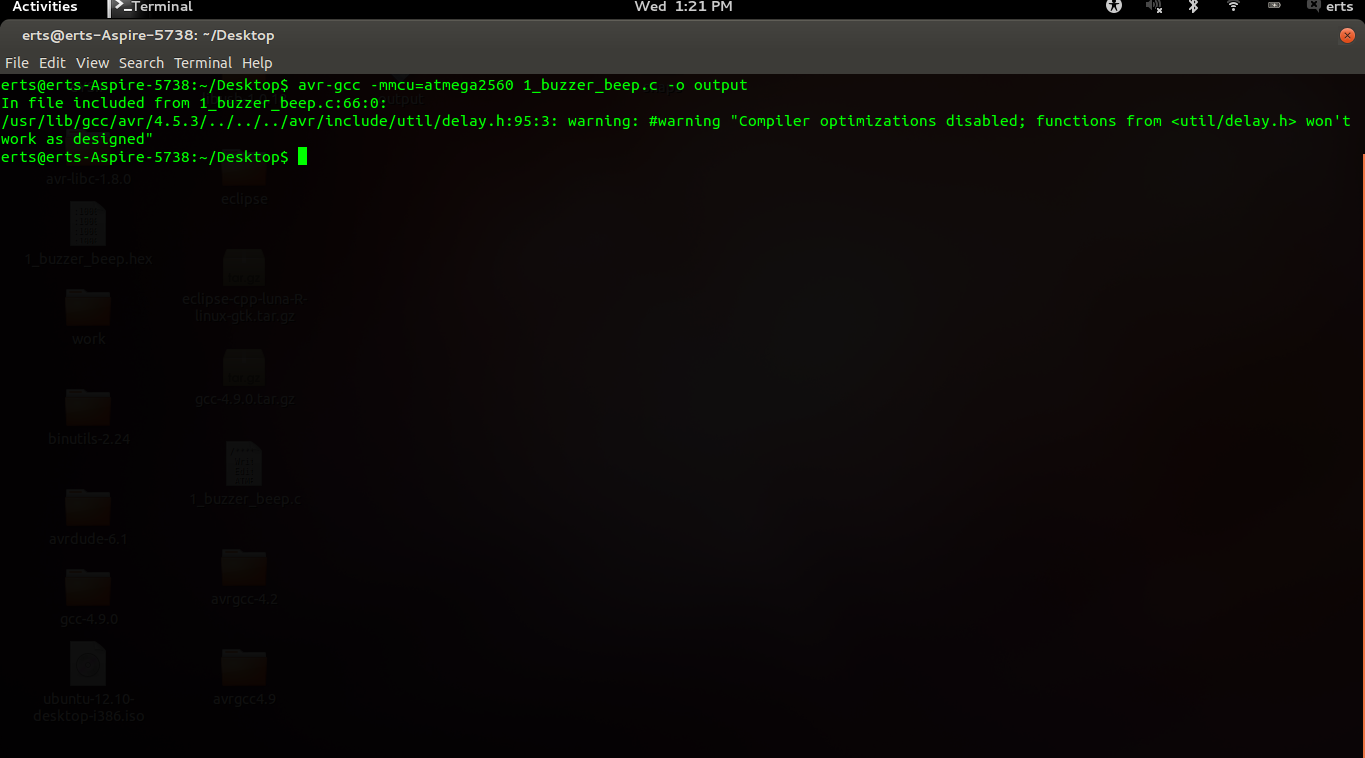
\includegraphics[scale=0.3]{f23}

\medskip

\subsection{Generation of the .hex file}

\medskip

To generate the .hex file type - 

\medskip

\framebox{\parbox{\dimexpr\linewidth-2\fboxsep-2\fboxrule}{avr-objcopy -O ihex some\_name source.hex}}

\medskip

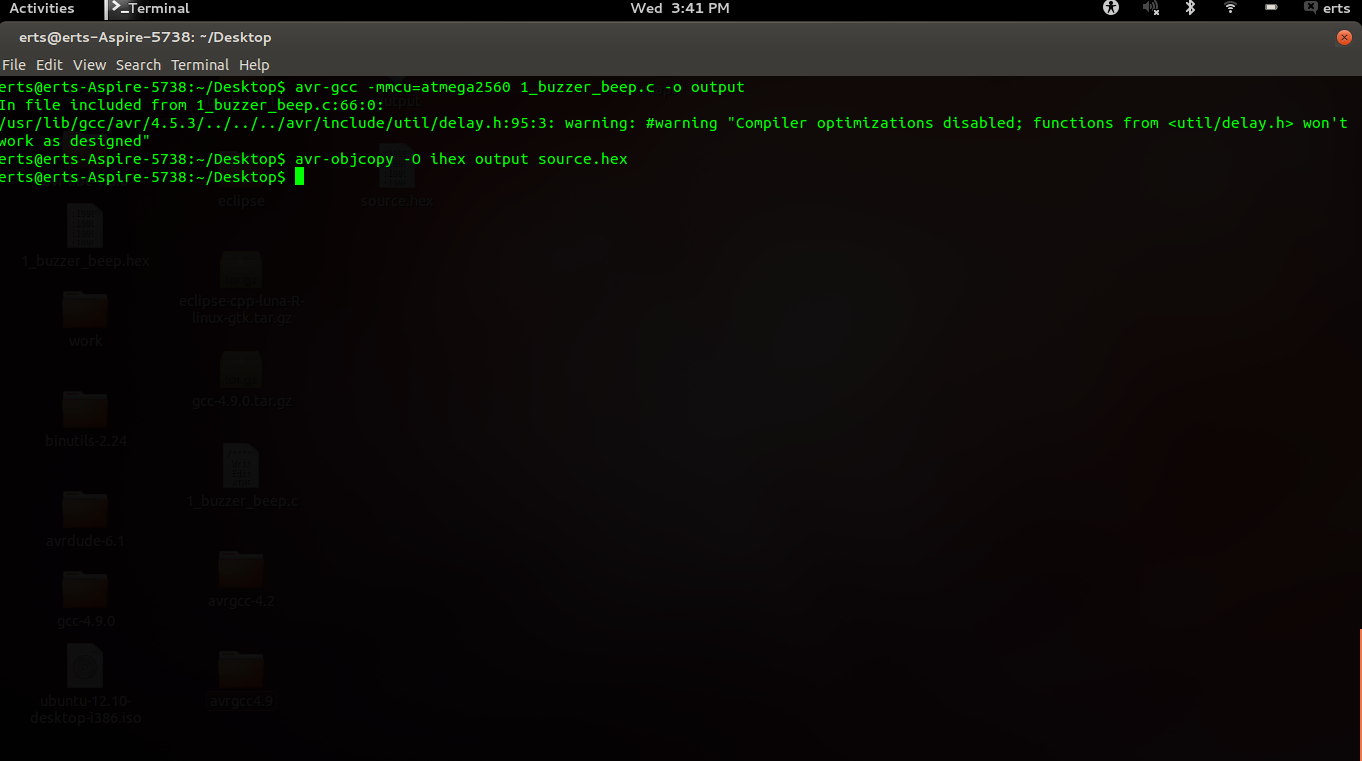
\includegraphics[scale=0.3]{f24}

\medskip


\subsection{Loading the .hex file}

\medskip

To load the .hex file on the Atmega2560 microcontroller using stk500v2 programmer type - 

\medskip

\framebox{\parbox{\dimexpr\linewidth-2\fboxsep-2\fboxrule}{sudo avrdude -c stk500v2 -p m2560 -P /dev/ttyACM0 -U flash:w:'/filepath/filename.hex':i}}

\medskip

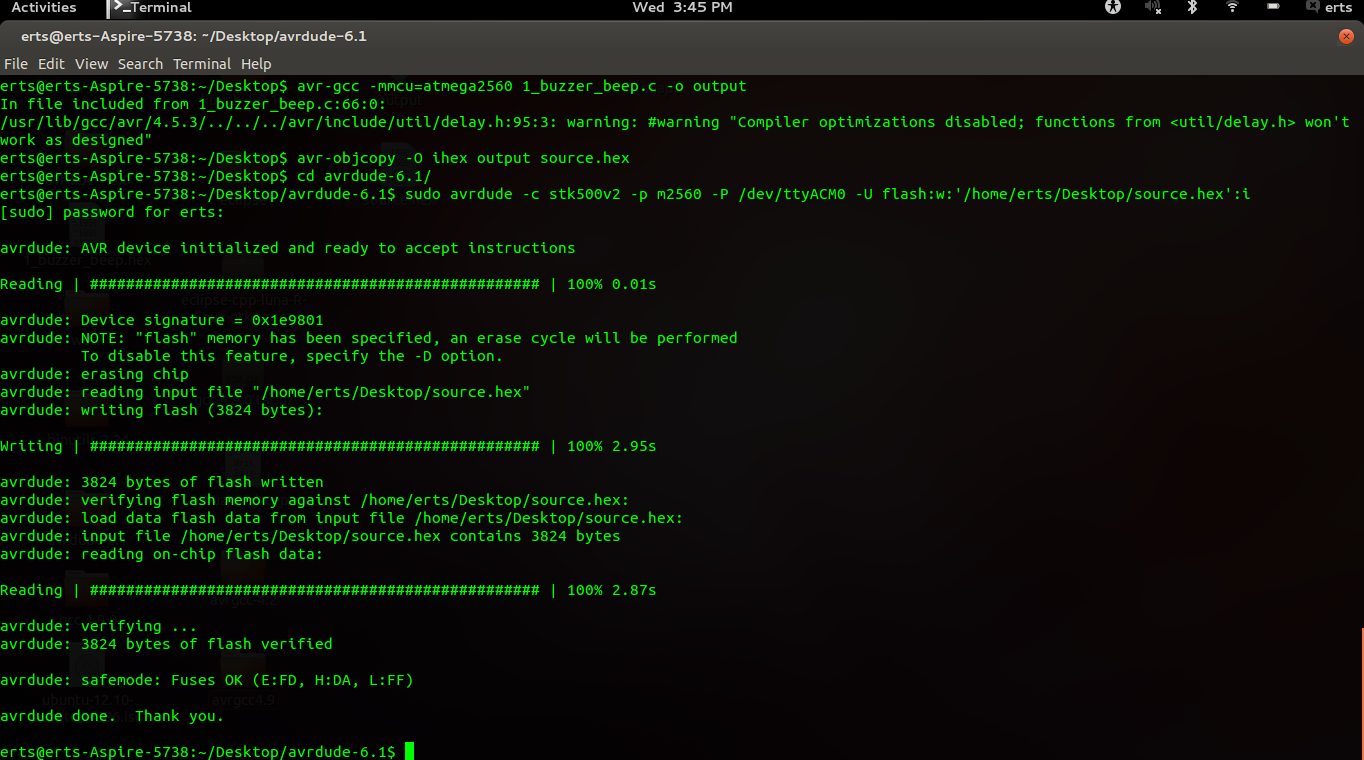
\includegraphics[scale=0.3]{f25}

\medskip

\Large{\textbf{Congratulations ! You have just completed the installation of Avrdude and loaded a .hex file on the Atmega2560 controller using the same.}}

\end{flushleft}

